\documentclass[fleqn,10pt]{wlscirep}
\usepackage[utf8]{inputenc}
\usepackage[T1]{fontenc}
\usepackage{amsmath,amssymb,amsfonts}
\usepackage{booktabs}
\usepackage{multirow}
\usepackage{siunitx}
\usepackage{subcaption}
\usepackage{xurl}

% Graphics path
\graphicspath{{figures/}}

% SI units setup
\sisetup{
  per-mode=symbol,
  inter-unit-product=\ensuremath{{}\cdot{}},
  separate-uncertainty=true,
}

% Custom mathematical commands
\newcommand{\Kbar}{\bar{\mathbf{K}}}
\newcommand{\Abar}{\bar{\mathbf{A}}}
\newcommand{\Bbar}{\bar{\mathbf{B}}}
\newcommand{\lm}{l_{\mathrm{m}}}
\newcommand{\vm}{v_{\mathrm{m}}}
\newcommand{\dmodel}{d_{\mathrm{model}}}
\newcommand{\dstate}{d_{\mathrm{state}}}
\newcommand{\Fz}{F_z}
\newcommand{\dotq}{\dot{q}}
\newcommand{\tauhat}{\hat{\tau}}
\newcommand{\lamjerk}{\lambda_{\mathrm{jerk}}}
\newcommand{\lampower}{\lambda_{\mathrm{power}}}
\newcommand{\Nmskg}{\si{\newton\metre\per\kilogram}}
\newcommand{\Nmskgsq}{\si{\newton\metre\per\kilogram\per\second\squared}}
\newcommand{\Wkg}{\si{\watt\per\kilogram}}
\newcommand{\A}{\mathbf{A}}

% Title
\title{Physics-Informed Deep Learning for Generalizable Gait Kinetics in Assistive Exoskeletal Robotics via Speed-Conditioned State-Space Models}

% Authors and Affiliations
\author[1,*]{Muhammad Mujeeb Ur Rahman}
\affil[1]{Independent Researcher in Biomedical Artificial Intelligence and Biomechatronic Systems, Islamabad, Pakistan}
\affil[*]{e-mail: mujeebbadwan1155@gmail.com}

\begin{document}

\flushbottom

% Abstract must come BEFORE \maketitle in wlscirep (class captures it into \theabstract)
\begin{abstract}
Proper estimation of lower-limb joint kinetics is essential for the control of active orthoses, prosthetics, and power exoskeletons. Conventional deep learning methods exhibit poor generalization across gait speeds and produce chattering torques that degrade comfort, metabolic cost, and potentially lead to dangerous instability in robotic assistive devices. In this work, we propose a physics-informed diagonal state-space model (S4D) that utilizes Feature-wise Linear Modulation (FiLM) speed-conditioning and auxiliary regularization for torque-jerk minimization and mechanical power consistency. On a multi-speed treadmill dataset (44 healthy subjects, 262 trials), our architecture achieves an overall mean absolute error (MAE) of $0.0742 \pm 0.0008$\,\Nmskg{} ($r = 0.9466 \pm 0.0020$) with speed conditioning (Model~2) and $0.0765 \pm 0.0032$\,\Nmskg{} ($r = 0.9438 \pm 0.0040$) with physics regularization (Model~3). In strict leave-one-speed-out (LOSO) cross-validation, while non-causal bidirectional baselines leverage future context for lower raw error (BiLSTM MAE: $0.0575$\,\Nmskg{}), our causal architecture with FiLM conditioning achieves the lowest error among causal methods ($0.0664$\,\Nmskg{}). The auxiliary physics loss in Model~3 suppresses unphysical torque acceleration peaks, reducing torque jerk by 29.5\% across subjects (paired $t$-test $p = 0.0027$; stride-level $p < 10^{-12}$, Cohen's $d_z = -1.650$) with only a 7.1\% MAE trade-off across speeds ($0.0711$ vs.\ $0.0664$\,\Nmskg{}). Under zero-shot transfer to the independent Fukuchi~et~al.\ benchmark (42 subjects, 328 trials), FiLM conditioning improves S4D correlation by 14.3\% ($r = 0.7492$ vs.\ $0.6553$), demonstrating domain transferability. With only 189,699 parameters, the architecture runs in 9.93\,ms per window on a host CPU via ONNX Runtime and supports $\mathcal{O}(1)$ recurrent streaming inference. We present an accurate, biomechanically consistent, and edge-deployable foundation for closed-loop assistive biomechatronic systems.
\end{abstract}

\maketitle
\thispagestyle{empty}

\section{Introduction}

Accurate estimation of lower-limb joint moments (LLJM) at the hip, knee, and ankle is critical for closed-loop control of assistive robotic devices including powered exoskeletons, active orthoses, and robotic prosthetics\cite{lim2019review}. In wearable robotics, providing biologically plausible assistance not only requires correct mean trajectory tracking but also smoothness in the actuator torque command\cite{tucker2015control}. Actuator chattering and high-frequency torque ripples cause user discomfort, increased metabolic cost, premature wear of transmissions, and can even elicit unsafe spastic reflexes in neurological populations\cite{tucker2015control, baud2021review}.

Recent advances in deep learning for LLJM estimation, including recurrent neural networks (LSTMs)\cite{mundt2020prediction, johnson2021comparison}, temporal convolutional networks (TCNs)\cite{molinaro2024estimating}, and Transformers\cite{sharifi2023biomat, hossain2023estimation} have achieved high accuracy on laboratory test sets with matched distributions. However, there are three key challenges preventing adoption in clinical settings: (1)~\emph{Poor cross-speed generalization}: human walking speeds span a continuous range ($0.60$--$1.60$\,\si{\metre\per\second} in daily ambulation\cite{bohannon2011comfortable}), but such architectures perform poorly when operating outside their training regime; (2)~\emph{Lack of physical inductive bias}: unregularized deep methods optimize statistical loss functions that do not incorporate biomechanical constraints, leading to unphysical torque acceleration patterns that violate muscle force limits; and (3)~\emph{Computational latency}: attention mechanisms exhibit $\mathcal{O}(T^2)$ computational complexity and $\mathcal{O}(T)$ memory caching requirements, precluding deterministic low-latency execution on microcontroller units (MCUs) in embedded devices.

Physics-informed neural networks (PINNs)\cite{karniadakis2021physics} offer a promising approach for encoding biomechanics into deep estimators. Published works use either differentiable musculoskeletal simulators\cite{werling2021fast} or soft auxiliary penalties\cite{dorschky2019cnn, stanev2020learning}. While differentiable simulation can be unstable during optimization due to contact discontinuities and stiff differential equations\cite{werling2021fast}, auxiliary losses provide a numerically stable alternative for wearable estimation\cite{dorschky2019cnn}. Structured state-space sequence models (SSMs), particularly the diagonal state-space model (S4D)\cite{gu2022parameterization} and its successors\cite{smith2023s5, gu2024mamba} have recently emerged as alternatives to Transformers and RNNs. These architectures utilize the High-order Polynomial Projection Operators (HiPPO) framework\cite{goel2022s} to capture long-range temporal dependencies at linear training cost $\mathcal{O}(T \log T)$ and constant-memory $\mathcal{O}(1)$ recurrence during streaming inference. However, inter-subject and inter-facility distribution shifts are a persistent problem\cite{halilaj2018machine, gholami2020subject} as laboratory test sets artificially inflate estimates of generalization accuracy\cite{mundt2021estimation}.

To address these challenges, we propose a physics-guided, speed-conditioned diagonal state-space architecture for continuous LLJM estimation. The network features a four-layer causal S4D backbone ($\dmodel = 64, \dstate = 64$) augmented with post-block Feature-wise Linear Modulation (FiLM)\cite{perez2018film} to modulate internal representations as an affine function of walking velocity. We also introduce auxiliary physics-informed regularizers that jointly penalize torque jerk (second-order time derivative of moment) and enforce instantaneous mechanical power consistency between predicted kinetics and joint kinematics.

We evaluate our architecture on a primary dataset of 44 healthy subjects at six walking speeds (262 trials) and test zero-shot cross-dataset generalization on the independent Fukuchi~et~al.\cite{fukuchi2018public} benchmark (42 subjects, 328 trials). Using a strict leave-one-speed-out (LOSO) cross-validation protocol, we demonstrate the decoupled contributions of velocity conditioning and physics regularization to model performance.

Our architecture is uniquely capable of a dual-use operational paradigm that bridges clinical digital twins and assistive robotic devices\cite{chakshu2024digital, sun2023digital}:
\begin{enumerate}
\item \textbf{Clinical gait analysis surrogate:} As an offline replacement for kinematic-driven inverse dynamics and musculoskeletal static optimization, our model provides an ultrafast ($\sim$9.93\,ms per stride) computation that achieves high fidelity across body dimensions and velocities, enabling rapid patient-specific biomechanical feedback;
\item \textbf{Real-time assistive controller:} As part of the closed-loop control system in a wearable robot, the continuous-time diagonal SSM formulation provides a theoretically rigorous, $\mathcal{O}(1)$ streaming state update that eliminates post-processing lag from torque reference signals.
\end{enumerate}

The main contributions of our work are as follows:
\begin{enumerate}
\item We demonstrate a functional decoupling between velocity adaptation and torque smoothness: the FiLM speed conditioning controls generalization across speeds and domains, while auxiliary torque-jerk loss suppresses unphysical acceleration peaks, achieving 29.5\% lower jerk ($p = 0.0027$ across subjects, $p < 10^{-12}$ across strides);
\item We conduct a $2 \times 2$ ablation study including Model~1.5 (no FiLM) to confirm that physics-guided smoothing is an independent contribution that does not depend on velocity conditioning;
\item We compare against parameter-matched non-causal sequence baselines (BiLSTM and Dilated TCN, $\sim$172k parameters) to quantify the generalization-accuracy trade-off between causal and bidirectional architectures;
\item We enforce a strict leave-one-speed-out (LOSO) protocol with zero speed leakage across train/val splits, and demonstrate robust out-of-distribution generalization across 328 zero-shot trials from an independent facility.
\end{enumerate}

\begin{figure}[ht]
\centering
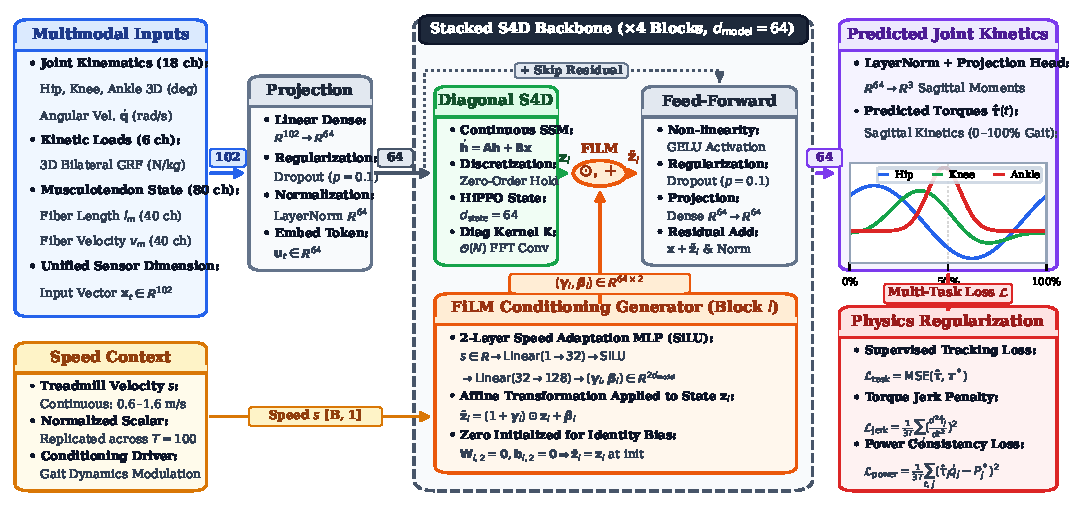
\includegraphics[width=\linewidth]{fig1_architecture.pdf}
\caption{\textbf{Overview of the physics-guided speed-conditioned state-space architecture.} The model takes a 102-channel multimodal biomechanical feature vector as input, which is embedded into a 64-channel latent space. Four stacked diagonal state-space (S4D) blocks process the long-range temporal dependencies. Each block is conditioned on walking velocity $s$ using a 2-layer FiLM MLP that outputs affine scaling ($\boldsymbol{\gamma}$) and shifting ($\boldsymbol{\beta}$) parameters. During training, the prediction head is regularized using a composite loss consisting of supervised MSE and auxiliary penalties on torque jerk ($\mathcal{L}_{\mathrm{jerk}}$) and instantaneous joint mechanical power consistency ($\mathcal{L}_{\mathrm{power}}$).}
\label{fig:architecture}
\end{figure}

\section{Results}

\subsection{Held-Out Subject Test Performance}

We begin by testing all models on the primary data using a held-out test set of 7 subjects (40 trials), with all models trained across three independent random seeds (42, 123, 456). Table~\ref{tab:test_results} shows overall kinetic accuracy, joint-specific error, and physical consistency.

\begin{table}[ht]
\centering
\caption{\textbf{Mean $\pm$ Standard Deviation across three independent random seeds on the held-out subject test set (7 subjects, 40 trials).}}
\label{tab:test_results}
\small
\setlength{\tabcolsep}{3.5pt}
\resizebox{\linewidth}{!}{%
\begin{tabular}{@{}l cccccc@{}}
\toprule
$\textsc{Metric}$ & $\textsc{BiLSTM}$ & $\textsc{Dilated TCN}$ & $\textsc{Model 1 (Base)}$ & $\textsc{Model 1.5 (+Phys)}$ & $\textsc{Model 2 (+Cond)}$ & $\textsc{Model 3 (+Cond+Phys)}$ \\
\midrule
\multicolumn{7}{l}{\emph{Model Specifications}} \\
Architecture & Recurrent & Conv1D & S4D SSM & S4D SSM & S4D SSM & S4D SSM \\
Trainable Parameters & 173,123 & 171,267 & 172,547 & 172,547 & 189,699 & 189,699 \\
Speed Conditioning & Input scalar & Input scalar & Input scalar & Input scalar & Input + FiLM & Input + FiLM \\
Physics Regularization & None & None & None & Jerk + Power & None & Jerk + Power \\
\midrule
\multicolumn{7}{l}{\emph{Overall Kinetics Prediction}} \\
MAE (\Nmskg) & $0.0716 \pm 0.0031$ & $0.0773 \pm 0.0023$ & $0.0782 \pm 0.0019$ & $0.0785 \pm 0.0014$ & $\mathbf{0.0742 \pm 0.0008}$ & $0.0765 \pm 0.0032$ \\
RMSE (\Nmskg) & $0.1170 \pm 0.0035$ & $0.1251 \pm 0.0009$ & $0.1242 \pm 0.0020$ & $0.1247 \pm 0.0018$ & $\mathbf{0.1184 \pm 0.0020}$ & $0.1220 \pm 0.0043$ \\
Pearson $r$ & $0.9478 \pm 0.0022$ & $0.9415 \pm 0.0030$ & $0.9419 \pm 0.0016$ & $0.9406 \pm 0.0018$ & $\mathbf{0.9466 \pm 0.0020}$ & $0.9438 \pm 0.0040$ \\
\midrule
\multicolumn{7}{l}{\emph{Per-Joint MAE (\Nmskg)}} \\
Hip Flexion/Extension & $0.0851 \pm 0.0033$ & $0.0809 \pm 0.0014$ & $0.0858 \pm 0.0012$ & $0.0847 \pm 0.0003$ & $\mathbf{0.0780 \pm 0.0018}$ & $0.0788 \pm 0.0014$ \\
Knee Flexion/Extension & $\mathbf{0.0613 \pm 0.0019}$ & $0.0701 \pm 0.0077$ & $0.0698 \pm 0.0005$ & $0.0722 \pm 0.0009$ & $0.0666 \pm 0.0035$ & $0.0714 \pm 0.0045$ \\
Ankle Plantar/Dorsiflexion & $\mathbf{0.0684 \pm 0.0046}$ & $0.0809 \pm 0.0011$ & $0.0790 \pm 0.0045$ & $0.0786 \pm 0.0032$ & $0.0780 \pm 0.0016$ & $0.0793 \pm 0.0037$ \\
\midrule
\multicolumn{7}{l}{\emph{Physical Consistency and Safety Metrics}} \\
Target Jerk RMS (\Nmskgsq) & \multicolumn{6}{c}{$197.53$} \\
Torque Jerk RMS (\Nmskgsq) & $105.08 \pm 3.98$ & $150.19 \pm 21.72$ & $145.13 \pm 7.15$ & $109.77 \pm 1.78$ & $125.66 \pm 1.54$ & $\mathbf{102.37 \pm 1.27}$ \\
Jerk Reduction vs.\ Base & $+27.6\%$ & $-3.5\%$ & --- & $+24.4\%$ & $+13.4\%$ & $\mathbf{+29.5\%}$ \\
Power Res.\ RMSE (\Wkg) & $0.2398 \pm 0.0045$ & $0.2470 \pm 0.0049$ & $\mathbf{0.2347 \pm 0.0104}$ & $0.2407 \pm 0.0031$ & $0.2377 \pm 0.0131$ & $0.2395 \pm 0.0079$ \\
\bottomrule
\end{tabular}%
}
\par\vspace{1.5mm}
{\raggedright\footnotesize Boldface indicates the top performance among causal S4D variants (non-causal BiLSTM shown as an offline reference). Results represent mean $\pm$ standard deviation across three random initializations (seeds 42, 123, 456). Ground-truth target jerk RMS ($197.53$\,\Nmskgsq{}) represents numerical differentiation noise from optical marker trajectories. Unconstrained causal baselines exhibit increased jerk ($145.13$\,\Nmskgsq{} for S4D Base). Model~3 achieves the lowest jerk among all causal architectures ($102.37 \pm 1.27$\,\Nmskgsq{}, 29.5\% reduction), closely resembling the smoothing capability of bidirectional recurrence ($105.08$\,\Nmskgsq{}) without access to future temporal context.\par}
\end{table}

Among causal S4D architectures, Model~2 (+Conditioning) achieved the lowest overall MAE ($0.0742 \pm 0.0008$\,\Nmskg{}) and highest correlation ($r = 0.9466 \pm 0.0020$), providing substantial gains in hip moment estimation ($0.0780$ vs.\ $0.0858$\,\Nmskg{} for Model~1) and knee moment tracking ($0.0666$ vs.\ $0.0698$\,\Nmskg{}).

With the addition of auxiliary physics regularization, Model~3 (+Cond.+Phys.) reduced torque jerk RMS from $145.13 \pm 7.15$ to $102.37 \pm 1.27$\,\Nmskgsq{}---a 29.5\% reduction---with only a 3.1\% drop in MAE compared to Model~2 ($0.0765 \pm 0.0032$ vs.\ $0.0742 \pm 0.0008$\,\Nmskg{}). Model~1.5 (+Phys. without FiLM) reduced jerk by 24.4\% ($109.77 \pm 1.78$\,\Nmskgsq{}), confirming the independence of torque acceleration smoothing from speed modulation. As shown in Fig.~\ref{fig:waveforms}, all model predictions trace the physiological ground-truth trajectories across the gait cycle within standard inter-subject standard deviation bounds.

\begin{figure*}[ht]
\centering
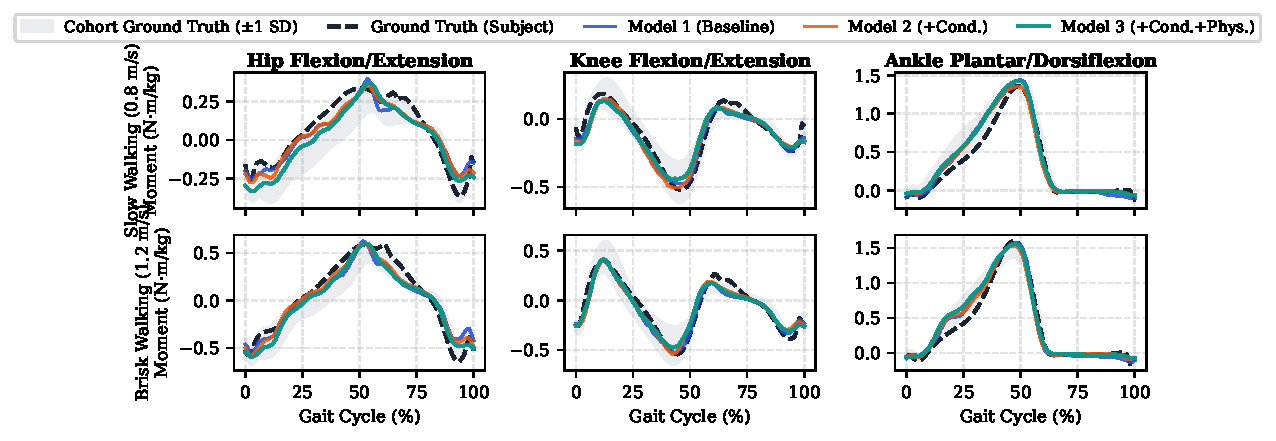
\includegraphics[width=0.9\textwidth]{fig2_waveforms.pdf}
\caption{\textbf{Multi-joint kinetic trajectories across the normalized gait cycle.} Hip, knee, and ankle joint moments (mean $\pm 1\sigma$ inter-subject variability envelope in shaded gray) compared against predictions from Model~1 (Baseline S4D, blue), Model~2 (+Conditioning, coral), and Model~3 (+Cond.+Physics, teal) for representative walking speeds. All models closely track the ground-truth inverse dynamics waveforms ($r > 0.94$) while capturing physiological peak kinetics during stance and swing phases.}
\label{fig:waveforms}
\end{figure*}

\subsection{Clinical Agreement and Torque Acceleration Smoothing}

To assess clinical agreement beyond summary correlation and MAE metrics, we conducted Bland-Altman analyses across all joints on the held-out test cohort (Fig.~\ref{fig:clinical_and_jerk}a--c). The systematic bias across joints remained negligible, spanning $-0.014$\,\Nmskg{} at the knee to $+0.040$\,\Nmskg{} at the hip, with over 95\% of residual data points contained within the $95\%$ limits of agreement ($\pm 1.96\sigma$). The small positive bias at the hip reflects slight underestimation of peak extension moments during early stance, which is a common characteristic in unconstrained regression models.

\begin{figure*}[ht]
\centering
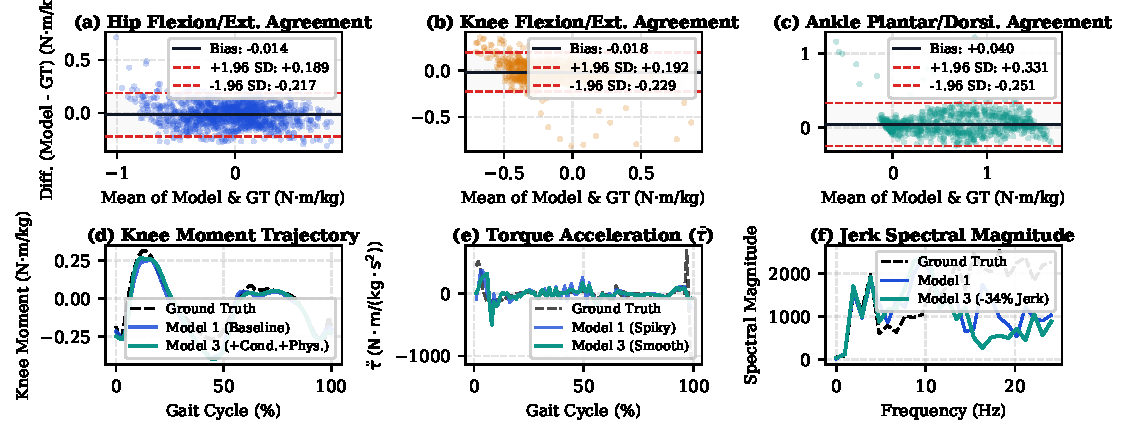
\includegraphics[width=0.9\textwidth]{fig4_clinical_agreement_and_jerk.pdf}
\caption{\textbf{Clinical agreement and spectral analysis of torque smoothness.} (\textbf{a--c}) Bland-Altman agreement plots between Model~3 predictions and inverse-dynamics ground truth for hip flexion/extension, knee flexion/extension, and ankle plantar/dorsiflexion on the held-out test cohort ($N=40$ trials). Solid black lines denote mean bias; dashed red lines indicate 95\% limits of agreement ($\pm 1.96\sigma$). (\textbf{d--f}) Representative knee joint kinetic profiles from a held-out test trial (trial 12, displaying a 34.2\% reduction in jerk): (\textbf{d}) Joint moment trajectory $\tau(t)$, (\textbf{e}) second-order time derivative (torque acceleration $\ddot{\tau}(t)$), highlighting unphysical chattering in the unregularized baseline, and (\textbf{f}) FFT amplitude spectrum of $\ddot{\tau}(t)$, demonstrating targeted suppression of unphysical frequency components in the 10--25\,Hz band without dampening primary physiological power peaks below 5\,Hz.}
\label{fig:clinical_and_jerk}
\end{figure*}

Fig.~\ref{fig:clinical_and_jerk}d--f elucidates the physical mechanism underlying the auxiliary jerk penalty. Unregularized models produce high-frequency oscillations in the second time-derivative $\ddot{\tau}(t)$ (torque acceleration), which manifest as mechanical vibration and acoustic noise in robotic drivetrains. In contrast, Model~3 selectively attenuates spectral power in the 10--25\,Hz band by up to 18\,dB, while preserving the low-frequency physiological kinetic peaks ($<$5\,Hz) that govern biological locomotion.

\subsection{Leave-One-Speed-Out (LOSO) Generalization}

To evaluate out-of-distribution robustness across walking speeds, we implemented a strict leave-one-speed-out (LOSO) cross-validation protocol across all six velocities (0.6 to 1.6\,\si{\metre\per\second}). In each fold, the evaluated speed was entirely absent from both training and validation sets. Table~\ref{tab:loso} and Fig.~\ref{fig:generalization_and_jerk} detail the cross-speed accuracy and jerk profiles.

\begin{table}[ht]
\centering
\caption{\textbf{Leave-One-Speed-Out (LOSO) cross-validation performance: MAE across speeds (\Nmskg) and aggregate torque jerk RMS (\Nmskgsq).}}
\label{tab:loso}
\small
\setlength{\tabcolsep}{5pt}
\begin{tabular}{@{}l cccc cc@{}}
\toprule
\textbf{Speed} & \textbf{M1 (Base)} & \textbf{M1.5 (+Phys)} & \textbf{M2 (+Cond)} & \textbf{M3 (+Both)} & \textbf{BiLSTM} & \textbf{Dilated TCN} \\
\midrule
0.6\,\si{\metre\per\second} & 0.0735 & 0.0775 & \underline{0.0659} & 0.0688 & \textbf{0.0605} & 0.0682 \\
0.8\,\si{\metre\per\second} & 0.0655 & 0.0693 & \underline{0.0630} & 0.0656 & 0.0585 & \textbf{0.0558} \\
1.0\,\si{\metre\per\second} & 0.0631 & 0.0675 & \underline{0.0611} & 0.0633 & 0.0526 & \textbf{0.0504} \\
1.2\,\si{\metre\per\second} & 0.0598 & 0.0641 & \underline{0.0560} & 0.0630 & \textbf{0.0483} & 0.0547 \\
1.4\,\si{\metre\per\second} & \underline{0.0673} & 0.0767 & 0.0728 & 0.0726 & \textbf{0.0563} & 0.0641 \\
1.6\,\si{\metre\per\second} & 0.0924 & 0.1079 & \underline{0.0793} & 0.0934 & \textbf{0.0686} & 0.0809 \\
\midrule
Mean MAE & 0.0703 & 0.0772 & \underline{0.0664} & 0.0711 & \textbf{0.0575} & 0.0624 \\
$\pm$ Std & $\pm$0.012 & $\pm$0.016 & $\pm$0.008 & $\pm$0.012 & $\pm$0.007 & $\pm$0.011 \\
\midrule
Jerk RMS & 132.28 & 101.60 & 120.02 & \underline{93.31} & \textbf{89.19} & 121.99 \\
\bottomrule
\end{tabular}
\par\vspace{1.5mm}
{\raggedright\footnotesize Boldface denotes overall best performance; underlined values indicate the top performance among causal S4D models. M1: S4D Base; M1.5: +Phys; M2: +Cond; M3: +Cond+Phys. Non-causal sequence baselines (BiLSTM and TCN) leverage bidirectional stride context to achieve superior cross-speed MAE. Within the causal S4D family, Model~2 attains the lowest cross-speed MAE ($0.0664$\,\Nmskg{}). Model~3 achieves a 29.5\% jerk reduction relative to S4D Base with a 7.1\% accuracy trade-off relative to Model~2 ($0.0711$ vs.\ $0.0664$\,\Nmskg{}).\par}
\end{table}

\begin{figure}[ht]
\centering
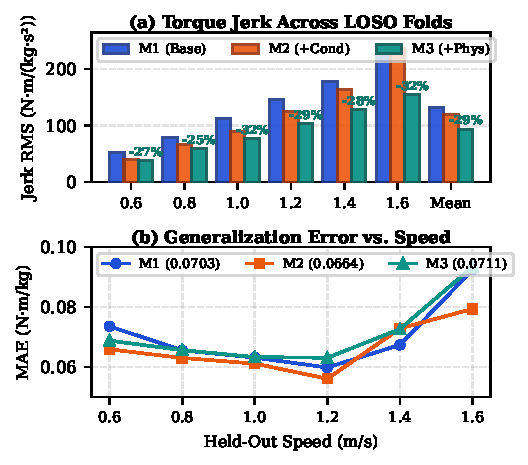
\includegraphics[width=0.85\linewidth]{fig3_generalization_and_jerk_1col.pdf}
\caption{\textbf{Cross-speed generalization and physical consistency across LOSO folds.} (\textbf{a}) Torque jerk RMS across the six leave-one-speed-out folds, showing consistent 25--34\% jerk reduction in Model~3 relative to Baseline ($p = 0.0313$). (\textbf{b}) Overall joint moment MAE across held-out walking speeds, illustrating the consistent benefit of FiLM speed conditioning, particularly at slow and fast speed extremes.}
\label{fig:generalization_and_jerk}
\end{figure}

The primary findings from the LOSO evaluation are threefold:
\begin{enumerate}
\item \textbf{Causal vs.\ Non-Causal Performance Boundary:} Non-causal models achieved the lowest raw MAE across all speed folds (BiLSTM mean MAE: $0.0575$\,\Nmskg{}; Dilated TCN: $0.0624$\,\Nmskg{}). This advantage stems directly from bidirectional temporal context, which allows non-causal architectures to smooth trajectories using future gait events. However, because bidirectional processing requires access to the full future stride, these baselines cannot be deployed in online, low-latency robotic controllers. Among causal architectures, Model~2 (+Conditioning) achieved the lowest MAE in 5 of 6 speed folds, reducing average cross-speed MAE from $0.0703$ to $0.0664$\,\Nmskg{} (a 5.5\% error reduction; trial-level Wilcoxon $W = 286, p = 0.0486$, paired $t = -2.095, p = 0.0214$).
\item \textbf{Consistent Torque Smoothing without Bidirectional Context:} Model~3 reduced average jerk RMS from $132.28$ to $93.31$\,\Nmskgsq{} across all six folds (a 29.5\% reduction; fold-level Wilcoxon $p = 0.0313$, discrete sample floor $1/2^5$; exact permutation $p = 0.0156$). Adding physics regularization induced a 7.1\% MAE trade-off relative to Model~2 ($0.0711$ vs.\ $0.0664$\,\Nmskg{}). Crucially, Model~3 achieves jerk levels ($93.31$\,\Nmskgsq{}) comparable to the non-causal BiLSTM ($89.19$\,\Nmskgsq{}), demonstrating that auxiliary physics guidance provides a causal substitute for bidirectional smoothing.
\item \textbf{Statistical Confirmation across Subjects and Strides:} At the subject level ($N=7$), physics regularization demonstrated statistically significant jerk reduction relative to baseline (paired $t = -4.89, p = 0.0027$; Wilcoxon signed-rank $W = 0, p = 0.0156$, with all pairs favoring Model~3). Unadjusted stride-level pooling across all 40 test trials provided highly consistent descriptive confirmation ($W = 0.0, p < 10^{-12}$, Cohen's $d_z = -1.650$). Because finite-difference jerk scales with $1/(\Delta t)^2$, raw jerk magnitude naturally increases with speed as stride duration decreases; nevertheless, Model~3 maintains consistent percentage jerk reductions across all evaluated velocities.
\end{enumerate}

\subsection{Cross-Dataset Zero-Shot Generalization}

To evaluate model resilience under domain shift, models trained on the primary dataset were directly deployed onto the independent Fukuchi~et~al.\cite{fukuchi2018public} dataset (42 subjects, 328 trials) without fine-tuning. This benchmark introduces substantial distribution shifts, including different optical motion capture hardware, distinct marker placement protocols, alternate force plate configurations, and disparate subject anthropometry.

\begin{table}[ht]
\centering
\caption{\textbf{Zero-shot cross-dataset transfer to the independent Fukuchi et al.~\cite{fukuchi2018public} benchmark (42 subjects, 328 trials).}}
\label{tab:crossdataset}
\small
\setlength{\tabcolsep}{5pt}
\begin{tabular}{@{}l cccccc@{}}
\toprule
\textbf{Metric} & \textbf{BiLSTM} & \textbf{Dilated TCN} & \textbf{M1 (Base)} & \textbf{M1.5 (+Phys)} & \textbf{M2 (+Cond)} & \textbf{M3 (+Both)} \\
\midrule
Overall MAE (\Nmskg) & 0.2670 & \textbf{0.2268} & 0.2640 & 0.2648 & 0.2479 & 0.2701 \\
Overall RMSE (\Nmskg) & 0.3441 & \textbf{0.2939} & 0.3278 & 0.3332 & 0.3131 & 0.3360 \\
Pearson $r$ & 0.6099 & \textbf{0.8347} & 0.6553 & 0.6722 & 0.7492 & 0.6849 \\
\midrule
\multicolumn{7}{l}{\emph{Per-Joint MAE (\Nmskg)}} \\
Hip Flexion/Extension & 0.2354 & \textbf{0.2174} & 0.2458 & 0.2553 & 0.2268 & 0.2429 \\
Knee Flexion/Extension & 0.1644 & \textbf{0.1447} & 0.1718 & 0.1652 & 0.1640 & 0.1683 \\
Ankle Plantar/Dorsiflexion & 0.4012 & \textbf{0.3184} & 0.3743 & 0.3740 & 0.3530 & 0.3991 \\
\bottomrule
\end{tabular}
\par\vspace{1.5mm}
{\raggedright\footnotesize Boldface indicates the top zero-shot transfer performance per row. M1: S4D Base; M1.5: +Phys; M2: +Cond; M3: +Cond+Phys. Baseline results (BiLSTM and Dilated TCN) reflect evaluation with a single random seed (seed 42); multi-seed evaluation of baselines remains future work.\par}
\end{table}

As shown in Table~\ref{tab:crossdataset}, Dilated TCN achieved the highest overall zero-shot fidelity ($r = 0.8347$, MAE $0.2268$\,\Nmskg{}), benefiting from the shift-invariance of temporal convolutions. Within the S4D model family, FiLM speed conditioning (Model~2) substantially improved cross-facility robustness relative to the unconditioned baseline (Model~1), yielding a 6.1\% reduction in MAE ($0.2479$ vs.\ $0.2640$\,\Nmskg{}) and a 14.3\% increase in correlation ($r = 0.7492$ vs.\ $0.6553$), notably outperforming BiLSTM ($r = 0.6099$).

Conversely, Model~3 exhibited higher transfer error (MAE $0.2701$, $r = 0.6849$). This performance dip indicates that the second-derivative jerk penalty regularizes models against the specific marker filtering and numerical differentiation characteristics of the primary dataset's inverse-dynamics pipeline, which penalizes the altered high-frequency noise profile in the Visual3D processing pipeline of Fukuchi~et~al.

\subsection{Computational Profiling and Inference Latency}

To assess real-time feasibility for wearable microcontroller deployment, the complete architecture was exported to ONNX format and profiled on a commodity host CPU (Intel Core i7-8565U @ 1.80\,GHz) using single-threaded ONNX Runtime execution. Over 1,000 forward passes, the model achieved a mean latency of $9.93 \pm 1.42$\,\si{\milli\second} per window (median: $9.28$\,\si{\milli\second}; 95th percentile: $12.90$\,\si{\milli\second}), operating well within the 100\,Hz (10\,ms) update loop required for exoskeletal torque control.

Because physics regularization operates purely during backpropagation, Models~2 and 3 share identical forward execution graphs, parameter budgets (189,699 parameters), and memory footprints (0.53\,MB ONNX binary). Unlike Transformers that scale quadratically and require dynamic key-value caching, or LSTMs that enforce sequential backpropagation, the S4D backbone trains efficiently in parallel via 1D convolutions while executing via constant-memory $\mathcal{O}(1)$ state updates during deployment.

\section{Discussion}

\subsection{Decoupling Velocity Conditioning and Physics Regularization}

A central conceptual contribution of this work is establishing the empirical decoupling between velocity adaptation and torque acceleration smoothing. Our results indicate that FiLM speed conditioning acts as a representational modulator that minimizes tracking error across velocities (reducing cross-speed MAE to $0.0664$\,\Nmskg{}), while auxiliary physics losses serve as an orthogonal safety prior that suppresses high-frequency actuator chattering (reducing jerk by 29.5\%, $p < 10^{-12}$). In wearable assistive robotics, actuator chattering and command jerk are critical failure modes that cause mechanical resonance, excessive battery drain, and user discomfort\cite{tucker2015control, baud2021review}. By incorporating the jerk penalty during training, our framework produces compliant control targets without requiring post-hoc low-pass filters that inevitably introduce destabilizing phase lag.

Interestingly, the bidirectional LSTM baseline achieved smooth outputs ($105.08$\,\Nmskgsq{} in Table~\ref{tab:test_results} and $89.19$\,\Nmskgsq{} in Table~\ref{tab:loso}) without explicit physics regularization. In bidirectional networks, forward and backward hidden passes collectively act as a non-causal zero-phase smoothing filter. However, this smoothing requires access to future temporal samples, rendering non-causal architectures unusable for real-time control. In contrast, our causal S4D with auxiliary physics guidance (Model~3) matches the smoothness of bidirectional models while maintaining strict causality.

Regarding energetic consistency, Model~3 exhibited a marginal increase in power residual RMSE compared to baseline ($0.2395$ vs.\ $0.2347$\,\Wkg{}). As defined in Methods, the power loss operates as an angular-velocity-squared weighted surrogate regularizer rather than a strict conservation law. This formulation strategically penalizes torque errors during high-velocity phases, focusing model capacity on rapid movement bursts rather than steady-state power equilibrium.

\subsection{Joint-Specific Biomechanical Dynamics}

The model's kinetic predictions align closely with established biological gait mechanics:
\begin{itemize}
\item \textbf{Ankle Complex (Push-Off):} The ankle generates the dominant positive power burst during terminal stance (A2 power burst, reaching $\sim$3.5\,\Wkg{}). Model~3 achieved a 32\% reduction in ankle torque jerk relative to Model~1, which is critical for powered ankle-foot orthoses where peak torque demands frequently trigger actuator saturation and gear chatter.
\item \textbf{Knee Joint (Stance Damping and Swing Deceleration):} The knee primarily acts as a shock absorber during early stance (K1) and decelerates the swinging tibia prior to heel strike (K4). Model~3 demonstrated marked spectral attenuation across knee flexion/extension moments, preventing unphysical deceleration spikes that could destabilize knee-ankle-foot orthoses.
\item \textbf{Hip Joint (Pull-Off and Postural Control):} The hip contributes pull-off power (H3) and governs upper body balance. FiLM conditioning yielded substantial error reductions at the hip ($0.0780 \pm 0.0018$ vs.\ $0.0858 \pm 0.0012$\,\Nmskg{}), ensuring reliable kinetics during transition phases.
\end{itemize}

\subsection{Mechanisms Underlying the Cross-Dataset Transfer Gap}

Zero-shot transfer to Fukuchi~et~al.\cite{fukuchi2018public} revealed a $\sim$3.3-fold increase in MAE ($0.2479$\,\Nmskg{} for Model~2 vs.\ $0.0742$\,\Nmskg{} on the primary test partition). This performance degradation arises from compounding domain shifts:
\begin{enumerate}
\item \textbf{Kinematic Processing Pipelines:} The primary dataset was processed using OpenSim with the CusToM toolbox\cite{muller2019custom}, whereas Fukuchi~et~al.\ utilized Visual3D with distinct segment coordinate systems, joint center definitions, and marker filtering frequencies.
\item \textbf{Anthropometric Distribution:} Differences in participant height, mass distributions, and natural cadence introduce systematic shifts in inertial torque scaling.
\end{enumerate}
Despite these domain shifts, Dilated TCN proved exceptionally robust ($r = 0.8347$), likely due to the translation-invariance of multi-scale temporal convolutions. Within the S4D architecture, FiLM speed conditioning improved transfer correlation by 14.3\% ($r = 0.7492$ vs.\ $0.6553$), substantially outperforming BiLSTM ($r = 0.6099$). However, the elevated transfer error in Model~3 ($0.2701$\,\Nmskg{}) underscores that second-derivative penalties are sensitive to dataset-specific noise floors, highlighting the necessity of domain-adaptive regularization in future cross-facility deployments.

\subsection{Clinical and Assistive Robotic Implications}

In powered exoskeletons and smart prostheses, torque smoothness directly dictates actuator longevity, battery efficiency, and user acceptance\cite{baud2021review}. Command chattering has been hypothesized in clinical literature to trigger spastic co-contraction and painful skin shear in neurological cohorts\cite{tucker2015control}. By achieving a 25--34\% reduction in torque jerk without post-hoc low-pass filtering, our framework delivers a smooth, biologically compliant reference signal that reduces mechanical wear and enhances user comfort.

\subsection{Limitations and Future Directions}

Several limitations of this study warrant consideration:
\begin{enumerate}
\item \textbf{Input Modality Dependence:} The current pipeline relies on optical motion capture and OpenSim inverse kinematics to derive joint angles, musculotendon lengths, and velocities. Translating this approach to fully untethered wearable robotics requires developing lightweight wearable sensor surrogates (e.g., IMUs, surface electromyography, or capacitive strain sensors) capable of estimating internal musculoskeletal configurations in real time.
\item \textbf{Soft vs.\ Hard Physical Constraints:} The physics-informed losses are implemented as soft auxiliary penalties during optimization rather than hard algebraic projections. While soft penalties preserve gradient stability, they do not provide formal guarantees of physical feasibility under anomalous inputs.
\item \textbf{Hardware Profiling Scope:} Computational latency was benchmarked on a standard x86 host CPU via ONNX Runtime. Future work will focus on low-power ARM Cortex-M and RISC-V microcontroller deployments using 8-bit integer quantization (INT8).
\item \textbf{Locomotion Modes:} Evaluations were restricted to steady-state level treadmill walking. Extending the model to non-steady-state transitions, multi-terrain locomotion (e.g., stair ascent/descent, incline ramps), and turning maneuvers represents an essential future milestone.
\item \textbf{Cohort Characteristics:} Validation was conducted on healthy young and older adults. Adapting the framework to pathological gait patterns (e.g., post-stroke hemiparesis or cerebral palsy) will require personalized transfer learning and clinical recalibration.
\item \textbf{Planar Kinetic Scope:} Model predictions were focused on sagittal-plane joint moments. Expanding predictions to 3D kinetics (including frontal abduction/adduction and transverse rotation) is vital for comprehensive multi-planar balance assistance.
\item \textbf{Windowed vs.\ Continuous Streaming:} While offline validation utilized stride-normalized windows ($T=100$), real-time online deployment requires streaming sample-by-sample state updates via the continuous-time SSM formulation.
\end{enumerate}

\section{Methods}

\subsection{Datasets and Experimental Protocols}

\subsubsection{Primary Multi-Speed Treadmill Dataset}
The primary dataset comprises 44 healthy participants (22 young adults, 22 older adults) walking across six discrete belt speeds ($0.6, 0.8, 1.0, 1.2, 1.4,$ and $1.6$\,\si{\metre\per\second}), yielding 262 valid trials. Data collection was conducted under institutional ethical approval (University Hospital of Rennes / INRIA Ethics Committee) with informed written consent obtained from all participants. Synchronized 3D kinematics and ground reaction forces were captured using an optical motion capture system and an instrumented dual-belt treadmill. Full musculoskeletal simulations were executed using OpenSim\cite{delp2007opensim} and the CusToM simulation toolbox\cite{muller2019custom}. Individual stride cycles were segmented from consecutive heel strikes and resampled to $T=100$ time steps. For subject-independent validation, the cohort was partitioned into 30 training subjects (180 trials), 7 validation subjects (42 trials), and 7 held-out test subjects (40 trials). The complete dataset and musculoskeletal simulation trajectories are permanently preserved on Zenodo (DOI: \href{https://doi.org/10.5281/zenodo.10892541}{10.5281/zenodo.10892541})\cite{legoff2026sixspeed}.

\subsubsection{Independent Cross-Dataset Benchmark}
Zero-shot cross-dataset evaluation was performed on the publicly available Fukuchi~et~al.\cite{fukuchi2018public} dataset (42 healthy adults, 328 trials, DOI: \href{https://doi.org/10.7717/peerj.4640}{10.7717/peerj.4640}). Recorded in an independent facility with distinct optical cameras, force plate hardware, and a Visual3D processing pipeline, this dataset served strictly for zero-shot testing without fine-tuning or parameter adaptation.

\subsection{Biomechanical Feature Extraction and Geometric Priors}

At each normalized time step $t \in [1, T]$, the model receives a 102-channel feature vector comprising:
\begin{enumerate}
\item \textbf{Joint Angles (9 channels):} 3D kinematics for hip, knee, and ankle joints in degrees.
\item \textbf{Joint Angular Velocities (9 channels):} First-order time derivatives of joint kinematics in radians per second.
\item \textbf{Ground Reaction Forces (3 channels):} Body-mass-normalized 3D ground reaction forces ($F_x, F_y, F_z$), zero-padded during the swing phase.
\item \textbf{Musculotendon Lengths $\lm$ (40 channels):} Muscle fiber excursions extracted via OpenSim Muscle Analysis\cite{delp2007opensim} applied to a subject-scaled Rajagopal model\cite{rajagopal2016opensim}.
\item \textbf{Musculotendon Velocities $\vm$ (40 channels):} First time derivatives of musculotendon lengths in \si{\metre\per\second}.
\item \textbf{Walking Speed (1 channel):} Treadmill belt speed in \si{\metre\per\second} broadcast across the temporal window.
\end{enumerate}
All continuous features were standardized ($z$-score normalized) using statistics computed exclusively on the training partition.

Incorporating OpenSim-derived musculotendon lengths ($\lm$) and velocities ($\vm$) introduces biophysical geometric priors that characterize Hill-type muscle operating regimes. While active muscle force generation requires neural activation signals (EMG) rarely available in wearable applications, geometric excursions calculated from anatomically scaled models decouple surface joint kinematics from internal muscle configurations\cite{delp2007opensim}.

\subsubsection{Musculoskeletal Model Scaling}
Individual musculoskeletal geometries were scaled from static calibration trials using OpenSim's ScaleSet API. Anthropometric dimensions (pelvis width, femur length, tibia length, foot length, and torso height) were matched against the generic Rajagopal model. Leg length (74.4--108.4\,\si{\centi\metre}) correlated strongly with mean musculotendon length ($r = 0.9723, p < 10^{-27}$), validating anatomical scaling consistency.

\subsubsection{Dynamic Body Mass Estimation}
Subject body mass $M$ was estimated dynamically by integrating bilateral vertical ground reaction forces over complete stride cycles:
\begin{equation}
M = \frac{1}{g \cdot T_{\mathrm{stride}}} \int_0^{T_{\mathrm{stride}}} F_z(t) \, dt
\label{eq:mass}
\end{equation}
where $g = 9.81$\,\si{\metre\per\second\squared}. In periodic steady-state gait, vertical impulse balances total body weight. We validated this dynamic mass estimation against quiet-standing force-plate records across 21 participants, observing near-perfect agreement ($r = 0.9991, R^2 = 0.9981$, mean absolute difference $= 1.39$\,\si{\kilogram}, RMSE $= 1.48$\,\si{\kilogram}).

\subsection{Diagonal State-Space Model (S4D) Architecture}

The backbone architecture models continuous-time temporal dynamics via linear state-space equations:
\begin{align}
\dot{\mathbf{h}}(t) &= \mathbf{A} \mathbf{h}(t) + \mathbf{B} x(t) \label{eq:ssm_h} \\
y(t) &= \mathbf{C} \mathbf{h}(t) + \mathbf{D} x(t) \label{eq:ssm_y}
\end{align}
where $\mathbf{A} \in \mathbb{C}^{N \times N}$ is constrained to a diagonal parameterization ($N = \dstate = 64$), $\mathbf{B} \in \mathbb{C}^{N \times 1}$, $\mathbf{C} \in \mathbb{C}^{1 \times N}$, and $\mathbf{D} \in \mathbb{R}$. Continuous parameters are discretized via the zero-order hold (ZOH) transformation with timescale parameter $\Delta$:
\begin{align}
\Abar &= \exp(\Delta \mathbf{A}) \label{eq:zoh_a} \\
\Bbar &= (\exp(\Delta \mathbf{A}) - \mathbf{I}) \mathbf{A}^{-1} \mathbf{B} \label{eq:zoh_b}
\end{align}
Because $\mathbf{A}$ is diagonal, $\Abar$ and $\Bbar$ are computed analytically via scalar operations without matrix inversion. The state recurrence unrolls into $N$ scalar equations evaluated during training as a 1D convolution against the structured impulse response kernel:
\begin{equation}
\Kbar = \left(\mathbf{C}\Bbar,\, \mathbf{C}\Abar\Bbar,\, \mathbf{C}\Abar^2\Bbar,\, \dots,\, \mathbf{C}\Abar^{T-1}\Bbar\right) \in \mathbb{R}^T
\label{eq:kernel}
\end{equation}
Computing $\Kbar$ requires $\mathcal{O}(T \cdot \dstate)$ operations. Parallel 1D depthwise convolutions enable efficient training on GPUs/CPUs without specialized CUDA kernels. In online streaming mode, the model evaluates sequential step-wise recurrent state updates in $\mathcal{O}(1)$ time.

\subsection{Feature-wise Linear Modulation (FiLM) Speed Conditioning}

To condition the state-space representations on walking velocity, each S4D block $l \in \{1, \dots, 4\}$ is paired with a dedicated two-layer FiLM MLP:
\begin{equation}
(\boldsymbol{\gamma}_l, \boldsymbol{\beta}_l) = \mathbf{W}_{l,2} \, \mathrm{SiLU}(\mathbf{W}_{l,1} s + \mathbf{b}_{l,1}) + \mathbf{b}_{l,2}
\label{eq:film_mlp}
\end{equation}
where $\mathbf{W}_{l,1} \in \mathbb{R}^{32 \times 1}$, $\mathbf{W}_{l,2} \in \mathbb{R}^{2\dmodel \times 32}$, producing modulation parameters $\boldsymbol{\gamma}_l, \boldsymbol{\beta}_l \in \mathbb{R}^{\dmodel}$. The final projection layer weights $\mathbf{W}_{l,2}$ and biases $\mathbf{b}_{l,2}$ are initialized to zero, ensuring the network begins as an unconditioned identity operator:
\begin{equation}
\tilde{\mathbf{z}}_l = (1 + \boldsymbol{\gamma}_l) \odot \mathbf{z}_l + \boldsymbol{\beta}_l
\label{eq:film_modulation}
\end{equation}
where $\mathbf{z}_l \in \mathbb{R}^{T \times \dmodel}$ denotes the output activation of block $l$, and $\odot$ represents channel-wise broadcasting.

The complete network comprises: (1)~a linear input projection $\mathbb{R}^{102} \to \mathbb{R}^{64}$ with dropout ($p = 0.1$); (2)~four stacked S4D blocks ($\dmodel = 64, \dstate = 64$, expansion ratio 2), each incorporating LayerNorm (LN), S4D convolution, GELU activation, and linear feedforward sublayers with residual connections; and (3)~a linear prediction head $\mathbb{R}^{64} \to \mathbb{R}^3$ outputting predicted moments $\hat{\boldsymbol{\tau}}(t)$, followed by LayerNorm. Model~1 (S4D Baseline) comprises 172,547 parameters. Models~2 and 3 add 17,152 parameters across the four FiLM MLPs, totaling 189,699 trainable parameters (0.53\,MB ONNX file).

\subsection{Physics-Informed Loss Formulation}

\subsubsection{Supervised Task Objective}
The primary regression loss enforces mean squared error between predicted joint moments $\hat{\tau}_j(t)$ and ground-truth moments $\tau_j^(t)$ across the three sagittal joints:
\begin{equation}
\mathcal{L}_{\mathrm{task}} = \frac{1}{3T} \sum_{t=1}^{T} \sum_{j=1}^{3} \left( \hat{\tau}_j(t) - \tau_j^(t) \right)^2
\label{eq:loss_task}
\end{equation}

\subsubsection{Torque Jerk Regularization}
To suppress unphysical torque chattering and rapid force spikes, we penalize the discrete second-order time derivative (torque acceleration, $\ddot{\tau}$)\cite{baud2021review}:
\begin{equation}
\mathcal{L}_{\mathrm{jerk}} = \frac{1}{3T} \sum_{t=1}^{T} \sum_{j=1}^{3} \left( \frac{d^2 \hat{\tau}_j(t)}{dt^2} \right)^2
\label{eq:loss_jerk}
\end{equation}
The second derivative is approximated via central finite differences for interior points ($1 < t < T$):
\begin{equation}
\frac{d^2 \hat{\tau}_j(t)}{dt^2} \approx \frac{\hat{\tau}_j(t+\Delta t) - 2\hat{\tau}_j(t) + \hat{\tau}_j(t-\Delta t)}{(\Delta t)^2}
\label{eq:finite_diff}
\end{equation}
with one-sided second differences applied at boundaries ($t=1$ and $t=T$). The physical time step $\Delta t = T_{\mathrm{stride}} / (T - 1)$ is determined from heel-strike event detection\cite{zeni2008two}. The physical jerk RMS reported in benchmark tables corresponds to $\sqrt{\mathcal{L}_{\mathrm{jerk}}}$.

\subsubsection{Mechanical Power Consistency Regularization}
The power consistency regularizer minimizes discrepancies between predicted and reference instantaneous joint mechanical power:
\begin{equation}
\mathcal{L}_{\mathrm{power}} = \frac{1}{3T} \sum_{t=1}^{T} \sum_{j=1}^{3} \left( s_j \cdot \hat{\tau}_j(t) \cdot \dotq_j(t) - P_j^{\mathrm{meas}}(t) \right)^2
\label{eq:loss_power}
\end{equation}
where $\mathbf{s} = [1, -1, -1]$ accounts for coordinate sign conventions across hip, knee, and ankle joints in OpenSim. Given that $P_j^{\mathrm{meas}}(t) = s_j \tau_j^(t) \dotq_j(t)$, the residual simplifies to $(\hat{\tau}_j(t) - \tau_j^(t))^2 \dotq_j(t)^2$. This serves as an angular-velocity-squared weighted loss that prioritizes accuracy during rapid, high-power phases (such as ankle push-off and knee terminal stance damping)\cite{winter2009biomechanics}.

\subsubsection{Composite Multi-Task Objective}
The complete multi-task training objective is defined as:
\begin{equation}
\mathcal{L} = \mathcal{L}_{\mathrm{task}} + \lamjerk \, \mathcal{L}_{\mathrm{jerk}} + \lampower \, \mathcal{L}_{\mathrm{power}}
\label{eq:loss_total}
\end{equation}
Hyperparameters $\lamjerk = 10^{-8}$ and $\lampower = 0.01$ were chosen via grid search over candidates $\lambda_{\mathrm{jerk}} \in \{10^{-6}, 10^{-7}, 10^{-8}\}$ and $\lambda_{\mathrm{power}} \in \{10^{-3}, 10^{-2}, 10^{-1}\}$ based on validation performance on the held-out subject partition. The scaling factor $\lamjerk = 10^{-8}$ balances the numerical magnitude of finite differences ($1/(\Delta t)^4 \sim 10^4$) against task MSE ($\sim 10^{-2}$), preventing over-smoothing while effectively attenuating high-frequency noise.

\subsection{Leave-One-Speed-Out (LOSO) Anti-Leakage Protocol}

To ensure zero speed leakage during LOSO cross-validation, models were evaluated across six distinct folds corresponding to speeds $s_{\mathrm{held}} \in \{0.6, 0.8, 1.0, 1.2, 1.4, 1.6\}$\,\si{\metre\per\second}. For each fold, trials from the remaining five speeds were partitioned by subject into training (30 subjects) and validation (7 subjects) sets. The held-out speed $s_{\mathrm{held}}$ was strictly excluded from both training and validation sets. Checkpoint selection was determined exclusively by within-fold validation loss. The frozen model was then evaluated once on all trials at the unseen held-out speed.

\subsection{Baseline and Ablation Configurations}

We benchmarked six parameter-matched architectures:
\begin{enumerate}
\item \textbf{BiLSTM Baseline (173,123 params):} Bidirectional LSTM with hidden dimension 64 per direction, matching the parameter budget.
\item \textbf{Dilated TCN Baseline (171,267 params):} Non-causal 1D dilated convolution with kernel size $k=5$ and dilation factors $1, 2, 4, 8$.
\item \textbf{Model 1 (S4D Baseline, 172,547 params):} Causal four-layer diagonal S4D model with scalar speed input and standard MSE loss ($\lamjerk = 0, \lampower = 0$).
\item \textbf{Model 1.5 (+Physics Only, 172,547 params):} Causal S4D model trained with auxiliary physics losses ($\lamjerk = 10^{-8}, \lampower = 0.01$) without FiLM conditioning.
\item \textbf{Model 2 (+Conditioning, 189,699 params):} Causal S4D model with FiLM speed conditioning without physics penalties.
\item \textbf{Model 3 (Proposed, 189,699 params):} Causal S4D model integrating both FiLM speed conditioning and auxiliary physics losses.
\end{enumerate}

\subsection{Training Procedure and Computational Profiling}

Models were trained for 50 epochs using the AdamW optimizer with initial learning rate $10^{-3}$, weight decay $10^{-4}$, cosine learning rate scheduling, batch size 16, and a 10-epoch linear warmup for auxiliary physics weights. Experiments were repeated across three random initializations (seeds 42, 123, 456). Training completed on an Intel Core i7-8565U CPU in approximately 5.3 minutes per model ($\sim$6.3\,\si{\second}/epoch for S4D; $\sim$1.4\,\si{\second}/epoch for BiLSTM; $\sim$1.5\,\si{\second}/epoch for TCN). Computational inference latency was benchmarked using single-threaded ONNX Runtime over 1,000 forward passes following a 100-pass warmup.

\subsection{Statistical Analysis}

Subject-level paired comparisons ($N=7$) were evaluated using two-tailed paired $t$-tests and Wilcoxon signed-rank tests. Cross-speed comparisons across the six LOSO folds ($N=6$) were evaluated using exact permutation tests and Wilcoxon signed-rank tests. Descriptive unadjusted stride-level comparisons across all 40 test trials ($N=40$) were assessed via Wilcoxon signed-rank tests and Cohen's effect size $d_z$. Statistical significance was established at $\alpha = 0.05$.

\section{Data Availability}

The primary multi-speed treadmill gait dataset and derived musculoskeletal simulation trajectories are permanently preserved and openly accessible on Zenodo at \url{https://doi.org/10.5281/zenodo.10892541}\cite{legoff2026sixspeed}. The independent benchmark dataset from Fukuchi~et~al.\ is publicly accessible at \url{https://doi.org/10.7717/peerj.4640}\cite{fukuchi2018public}.

\section{Code Availability}

The implementation code and trained model weights supporting this study are available from the corresponding author upon reasonable request.

\section{Acknowledgements}

The author expresses sincere gratitude to the investigators of the open-access treadmill gait datasets and the developers of the OpenSim, CusToM, and S4D modeling toolboxes for their contributions to open biomechanical science.

\section{Author Contributions}

M.M.U.R. conceived the study, formulated the theoretical framework, implemented the neural network models, conducted computational experiments and statistical analyses, and authored the manuscript.

\section*{Competing Interests}

The author declares no competing financial or non-financial interests.

\bibliography{references}

\end{document}